\documentclass[12pt, a4paper]{article}  
\title{An Empirical Analysis on Japan's Environmental Kuznets Curve}
\author{Masaru Komaya, Takahiro Kawano}
\date{December 22, 2016}
\usepackage[margin=1in]{geometry}
\usepackage[dvipdfmx]{color}
\usepackage[dvipdfmx]{graphicx}
\usepackage{threeparttable}
\usepackage{booktabs}
\usepackage{multirow}
\usepackage{bm}
\usepackage{amsmath}
\usepackage{amsfonts}
\usepackage{ascmac}
\usepackage{apacite}
\usepackage{url}
\linespread{1.5}
\renewcommand\thefootnote{\arabic{footnote})}
\begin{document}
\maketitle
\newpage
\tableofcontents
\newpage
%以下本文
\section{Abstract}
The theory of Environmental Kuznets Curve (EKC) shows an relationship between \textstyle{$CO_2$} emissions and GDP per capita. However, this curve is not enough model to forecast \textstyle{$CO_2$} emissions precisely. Based on this theory, we try to reform the original EKC model for the purpose of forecasting. Specifically, we add more two types of factors: a ratio of fossil fuel energy consumption in total and Japanese population in urban area. Our estimated model was based on data which is from 1962 to 2005. By using the estimated model, we try static forecast, which is intended to forecast amount of \textstyle{$CO_2$} emissions next year. Results of static forecast from 2005 to 2010 are shown in this paper. \\
Broadly speaking, our model shows good performance in forecasting one year ahead, except for the period of the financial crisis happened in 2008. In addition to forecasting, there is a positive correlation between growth rate of \textstyle{$CO_2$} emissions and growth rate of fossil fuel energy consumption in total. Intuitively, \textstyle{$CO_2$} emissions increase as a ratio of fossil energy consumption in total increases. Secondly, there is a negative correlation between growth rate of \textstyle{$CO_2$} emissions and growth rate of population in urban area. It implies that population concentration in urban area has potential to reduce \textstyle{$CO_2$} emissions. 
\newpage

\section{Motivation}
 The Intergovernmental Panel on Climate Change (IPCC) issued a global climate assessment in 2007. According to the research by IPCC, \textstyle{$CO_2$}, more than any other factors, has contributed the most to global warming between 1750 and 2005. To tackle the global warming issue, it is important to forecast how \textstyle{$CO_2$} emissions will be in the future. Any political and economic decisions should be based on how situations are going to be in the future. In this sense, forecast of future \textstyle{$CO_2$} becomes crucial information for making decisions, and it would contribute to making policy for global warming. In this paper, we focus on Japan’s case, for contributing to policy making by the Japanese government.  

\section{Problems to be solved}
According to the Environmental Kuznets Curve(EKC), there is a relationship between \textstyle{$CO_2$} emissions and GDP per capita. In the early stages of economic growth degradation and pollution increase, but beyond some level of income per capita, the trend reverses. After the turning point of high-income levels, economic growth leads to environmental improvement. This curve implies inverted U-shaped function. However, this curve is not enough to forecast future \textstyle{$CO_2$} emissions precisely, since EKC has only the factor of GDP to explain \textstyle{$CO_2$} emissions. To deal with it, we add other factors and try to forecast future \textstyle{$CO_2$} emissions more precisely.


\section{Literature Review}
Shahbaz et al\footnote{Testing the Environmental Kuznets Curve Hypothesis in Portugal. Retrieved from \url{https://www.econjournals.com/index.php/ijeep/article/viewFile/1126/653}} (2015) investigated the reation between the emissions of \textstyle{$CO_2$} and GDP.  In the paper they proposed the following model; 
\begin{equation}
\begin{split}
\ln{(CO_2)}_{t}&=\beta_1+\beta_{ENC}\ln{(ENC)}_{t}+\beta_{GDP}\ln{(GDP)}_{t}+\beta_{GDP^2}(\ln{(GDP)}_{t})^2\\
&+\beta_{TR}\ln{(TR)}_{t}+\beta_{URB}\ln{(URB)}_{t}+\varepsilon_{t}
\end{split}
\end{equation}
where  \textstyle{$CO_2$}:\ emission of \textstyle{$CO_2$}  in Portugal, $ENC$:\ energy consumption, $GDP$:\ real GDP, $GDP^2$: square of GDP,\  $TR$:\ trade openness, and $URB$:\ urbanization.  $\varepsilon$:\ error term.\\
ln stands for the natural log and the subscript $t$ is years.\\
Using the modelling above, they estimated the long run equilibrium based on Error Correction Model (ECM).  The way of obtaining the ECM shall be mentioned in following chapter.\\

\section{Approach}
Based on the model (1), we analyse the Japan's EKC with long-run and short-run modelling.  Similar to (1), we employ Japanese GDP, urban population and energy consumption as variables to explain the \textstyle{$CO_2$} emissions.  Here, we omit the trade openness as one variable.  In this paper, we would like to focus on the forecast of future \textstyle{$CO_2$} emissions since it might be statistically insignificant to analyse each coefficient of variables due to multicolinerarity. 

\section{Dataset}
Since the geographical area of this analysis is limited to Japan, all the data is regarding only Japan from 1960 to 2010.  \textstyle{$CO_2$} represents per capita \textstyle{$CO_2$} emissions, $GDP$, per capita real $GDP$,  $ENC$, the percentage of fossil fuel energy consumption in total, $URBP$, urban population in total, respectively.\\
\textstyle{$CO_2$}: Japanese annual  \textstyle{$CO_2$}  emissions  per  capita from  World  Bank\footnote{\url{http://data.worldbank.org/indicator/EN.ATM.CO2E.PC?locations=JP}}.  (metric tonnes per capita)\\
$GDP$: Japanese annual Real  $GDP$  per  capita from  FRED\footnote{\url{https://fred.stlouisfed.org/series/JPNRGDPR}} (Federal  Reserve  Economic  Data)  at 2011 U.S. Dollars\\
$ENC$: Japanese annual percentage of fossil fuel energy consumption in total from World Bank\footnote{\url{http://data.worldbank.org/indicator/EG.USE.COMM.FO.ZS}}\\
$URBP$: Japanese population in urban area \footnote{A population of at least 50,000, a  percentage of non-agricultural workers of at least 75\%, at least as many daytime occupants as nighttime ones, no more than 30\% of the population commuting out, and no more than 15\% commuting to another central city} at the year from World Bank\footnote{\url{http://data.worldbank.org/indicator/SP.URB.TOTL?locations=JP}}\\

\section{Methogology}
As time series data are mostly following non-stationarity, it is basically impossible to make a significant analysis based on the non-stational data.  However, our analysis is supposed to construct the ECM, which assumes that the original series of independent variables are nonstationary.  Whether the series are following stationarity or non-stationarity is tested with Augumented Dicky-Fuller (ADF) test\footnote{\[y_t=(\delta-1)y_{t-1}+\varepsilon_t\]
$$H_0: \delta=1, H_a:\delta\leq 1$$}. First, we generate the modelling as follows;
\begin{equation}
\begin{split}
\ln{(CO_2)}_{t}&=\beta_1+\beta_{{CO_{2}}_{t-1}}\ln{(CO_2)}_{t-1}+\beta_{GDP}\ln{(GDP)}_{t}+\beta_{GDP^2}(\ln{(GDP)_{t}})^2\\
&+\beta_{URBP}\ln{(URBP)}_{t}+\beta_{ENC}\ln{(ENC)}_{t}+\beta_{trend}t+\varepsilon_{t}
\end{split}
\end{equation}
Where $\ln$ represents the natural log form, $t$ is trend, $\varepsilon$ is error term, the subscript $t$ is years\\
\\
After modelling (2), the residuals, $\varepsilon_{t}$, will be generated from the estimation.   Then, the ADF test for the residuals is implemented to assume that the residuals follow the stationarity, which is considered to be cointegrated.  To adjust the gap between actual and estmated values, we generate the ECM for the long-run equilibrium.\\
\\
In the short-run, the following model is employed.
\begin{equation}
\begin{split}
\varDelta{\ln{(CO_2)}_{t}}&=\beta_1+\beta_{GDP}\varDelta{\ln{(GDP)}_{t}}+\beta_{GDP^2}\varDelta{(\ln{(GDP)_{t}})^2}\\
&+\beta_{URBP}\varDelta{\ln{(URBP)}_{t}}+\beta_{ENC}\varDelta{\ln{(ENC)}_{t}}+\beta_{ECN}ECM_{t-1}+\varepsilon_{t}
\end{split}
\end{equation}
Where let $\varDelta$ denote the difference, $s.t. \varDelta y_t=y_t-y_{t-1}$, $EMC_{t-1}$ is the first lagged value of the residual from (2).\\
In a sense, the model (3) is trying to estimate the short-run equilibrium including the long-run effect of the previous year.\\
Notice that we omit the effect of \textstyle{$CO_2$} emissions at previous year and the statistical reason is shown in the empirical results.  

\section{Empirical Results}
First, we regress the model (2) to obtain the long-run equilibrium: In other words, we try to genertate the Error Correction Model (ECM).  The residuals of model (2) has passed the all tests in the Table \ref{model2}.  The t-values of all independent variables, except for constant, show statistically high value---The null hypothesis, each coefficient of independent variables=0, is rejected even at 1 percentage critical value.\\
In order to generate the ECM, we need to assume that the residuals from model (2) has to follow the stationarity.  Then, we implement the ADF test for the residuals with constant and two lags

\begin{table}[h]
  \caption{Modelling $\ln{(CO_2)}$ by OLS}
  \label{model2}
  \centering
  \begin{tabular}{lrrrrr}
    \hline
   Variable    &           Coefficient & Std.Error & t-value &  t-prob  & Part.$R^2$\\
\hline\hline
$\ln{(CO_2)}_1$    &    0.544532  &  0.05040   &  10.8  & 0.0000 &  0.7594\\
Constant      &       -5.92426  &    3.717 &   -1.59 &  0.1195  &   0.0643\\
$\ln{(GDP)}$     &       4.15775   &   0.9750  &    4.26  &  0.0001  &   0.3295\\
$(\ln{(GDP)})^2$   &   -0.183758  &  0.05064  &   -3.63  &  0.0009  &   0.2625\\
$\ln{(URBP)} $  &       -1.32941 &    0.1756 &    -7.57 &  0.0000  &  0.6076\\
$\ln{(ENC)} $     &      1.72165  &   0.2080   &   8.28  & 0.0000  &  0.6494\\
Trend       &        0.0130490 &   0.002307  &   5.66 &  0.0000  &   0.4637\\
\hline
sigma     &          0.0210812 &   RSS           &  0.016443412 &\\
$R^2$       &           0.995805 &  F(6,37) =   & 1464 [0.000]** &\\
Adj.$R^2$   &           0.995125  & log-likelihood   &     111.191 & \\
no. of observations    &    44 &  no. of parameters    &       7 & \\
mean(Y)      &         2.01501 & se(Y)      &        0.301937 & \\
\hline
AR 1-2 test:   &   F(2,35)   = & 0.72568 [0.4911]    & \\
ARCH 1-1 test: &   F(1,42)   = & 0.88624 [0.3519]  &\\
Normality test:  & $Chi^2(2)$  =  & 2.5051 [0.2858]  & \\
Hetero test:     & F(11,32)  = &  0.79366 [0.6449]  & \\
RESET23 test:   &  F(2,35)   = &  1.8763 [0.1682]  & \\
    \hline
  \end{tabular}
\end{table}


\begin{figure}[h]
  \begin{center}
    \caption{Graphics of model (2) actual and fitted (1962-2005)}
    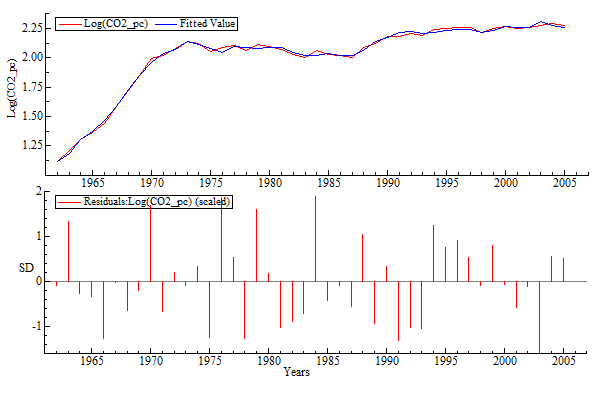
\includegraphics[scale=0.8]{fig1.png}
    \label{fig1} 
  \end{center}
\end{figure}

\begin{table}[h]
  \caption{ADF test for residuals with the intercept and two lags}
  \label{adf3}
  \centering
  \begin{tabular}{crrr}
    \hline
   Variable  & Std. Error & t-value\\
\hline\hline
$residuals_1$     &   -1.3704  &    0.31763  &    -4.3144\\
Constant    &   -0.00068595  &  0.0031450  &   -0.21811\\
$Dresiduals_1$ &    0.19736   &   0.24948  &    0.79106\\
$Dresiduals_2$  &     0.11245  &    0.16582  &    0.67816\\
    \hline
**$5\%=-2.934$, & *$1\%=-3.597$
  \end{tabular}
\end{table}

\newpage

Then, we can obtain the following ECM and we can assume that all coefficient is significant;\\
\[
\begin{split}
ECM =& \ln{(CO_2)} + 13.007 - 9.12852*\ln{(GDP)} + 0.403448*(\ln{(GDP)})^2 \\
&- 3.77995*\ln{(ENC)}+ 2.91877*\ln{(URBP)} - 0.0286496*Trend
\end{split}
\]
WALD test\footnote{WALD test is to assume that the all coefficient is significant.}: $Chi^2(5)$ =$ 1314.83 [0.0000]$ **


The table \ref{tb:model2} shows the results of model (3). Correlation coefficients of $\varDelta\ln(CO_2)$ is positively significant and that of $\varDelta(\ln(CO_2))^2$ is negatively significant. This results are consistent with the theory of EKC which implies inverted U shaped curve. \\
The unit of all variables except $ECM_1$, is first difference of log, which means growth rate of the variables. The table\ref{tb:model2} shows that correlation coefficient of $\varDelta\ln(URBP)$ is -1.4. When 1 unit of $\varDelta\ln(URBP)$ increases, 1 unit of $\varDelta\ln(CO_2)$ decreases. In this case, the unit of $\varDelta\ln(URBP)$ is growth rate. Therefore, 1 percent increase of growth rate in URBP leads to 1.4 percent decrease in \textstyle{$CO_2$} emissions. In the same interpretation, 1 percent increase of growth rate in ENC leads to 1.8 percent increase in \textstyle{$CO_2$} emissions. However, there is possibly a problem of multicollinearity. We should not conclude that correlation coefficient precisely represents effect size of each factor on \textstyle{$CO_2$} emissions.  
The figure \ref{fig3} shows actual time series data, estimated values and the residuals.\\  
\\
The (3) model passed all misspecification tests. Judging from the results of misspecification tests, we can keep an important assumption that residuals are at random. This assumption is quite important for precise and rigorous forecast. Therefore, the results of misspecification tests indicate that the model has high credibility in terms of forecasting. \\
\\
Figure \ref{fig5} shows the results of forecasting based on model (3). Based on our estimated model, we use static forecast to forecast 1 year ahead in the period from 2006 to 2010. Visually, most actual values are fell into 95 percent estimated intervals. In 2008 and 2009, actual values are out of the estimated intervals. We interpret it is because of the financial crisis.




\begin{figure}[h]
  \begin{center}
    \caption{Graphics of model (3) actual and fitted (1962-2005)}
    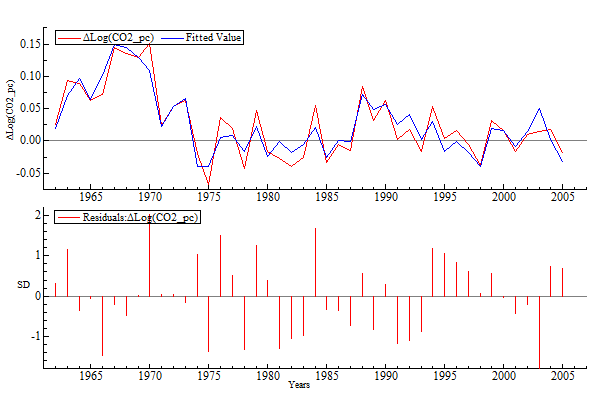
\includegraphics[scale=0.8]{fig3.png}
    \label{fig3} 
  \end{center}
\end{figure}

\begin{figure}[h]
  \begin{center}
    \caption{Graphics of model (3) residual analysis (1962-2005)}
    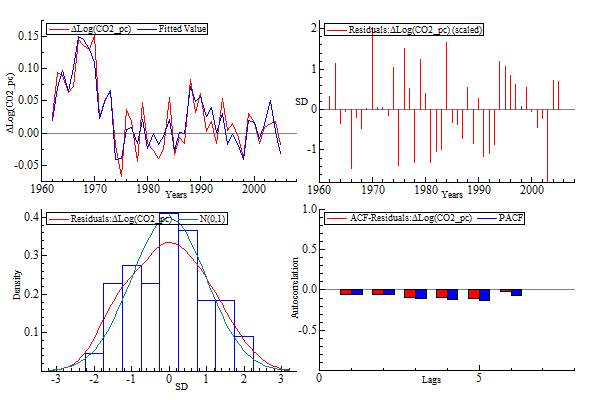
\includegraphics[scale=0.8]{fig4.png}
    \label{fig4} 
  \end{center}
\end{figure}



\begin{figure}[h]
  \begin{center}
    \caption{Graphics of Second model 1-step forecasting (2005-2010)}
    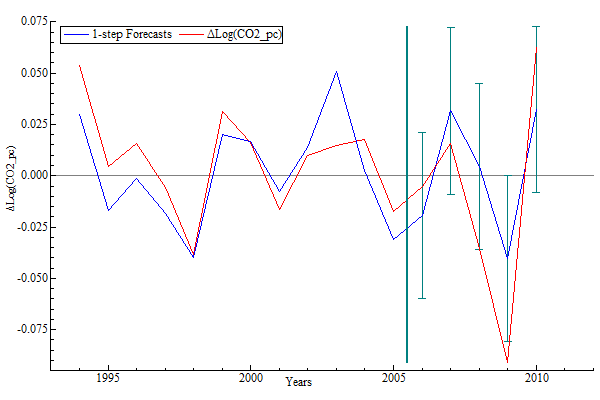
\includegraphics[scale=0.8]{fig5.png}
    \label{fig5} 
  \end{center}
\end{figure}


\newpage


\begin{table}[h]
  \caption{Modelling $\varDelta{\ln{(CO_2)}}$ by OLS}
  \label{tb:model2}
  \centering
  \begin{tabular}{lrrrrr}
    \hline
   Variable    &           Coefficient & Std.Error & t-value &  t-prob  & Part.$R^2$\\
\hline\hline
Constant           &            0.0146079   & 0.008165  &   1.79  & 0.0816 &  0.0777\\
$\varDelta{\ln{(GDP)}}$     &       3.82427   &   1.758  &   2.18 &  0.0359&   0.1108\\
$\varDelta{(\ln{(GDP)})^2}$   &   -0.162509 &   0.09309 &   -1.75 &  0.0889&   0.0742\\
$\varDelta{\ln{(URBP)}}$  &    -1.53139  &   0.4958 &   -3.09 &  0.0037&   0.2007\\
$\varDelta{\ln{(ENC)}}$      &      1.87824  &   0.2923  &   6.43 &  0.0000 &  0.5208\\
$ECM_1$            &              -0.418739 &   0.06162 &   -6.80  & 0.0000 &  0.5486\\
\hline
sigma       &        0.0204602 & RSS    &          0.0159075739&\\
$R^2$      &            0.866275&  F(5,38) =   &  49.23 [0.000]**&\\
Adj.$R^2$     &          0.84868 & log-likelihood     &    111.92&\\
no. of observations &       44 & no. of parameters &          6&\\
mean(Y)         &    0.0267854  &se(Y)    &           0.0525971&\\
\hline
AR 1-2 test:   &   F(2,36)   = & 0.75686 [0.4765]   &&\\
ARCH 1-1 test: &   F(1,42)   =  & 1.5204 [0.2244]  &&\\
Normality test:  & $Chi^2(2)$  =  & 1.5076 [0.4706]  &&\\
Hetero test:    &  F(10,33)  = & 0.27523 [0.9825]  &&\\
Hetero-X test:  &  F(20,23)  = & 0.48425 [0.9471]  &&\\
RESET23 test:   &  F(2,36)   = & 0.11529 [0.8914]  &&\\
    \hline
  \end{tabular}
\end{table}


\section{Concluding Remarks}
We conclude that the model (3) performs well to forecast one year ahead, except for the period of the financial crisis happened in 2008. Due to the world’s financial crisis, amount of \textstyle{$CO_2$} emissions decreased, as Japan’s GDP per capita declined between 2008 and 2009.
 Besides the forecasts, we found that there is a positive correlation between growth rate of \textstyle{$CO_2$} emissions and growth rate of fossil fuel energy consumption in total. Intuitively, \textstyle{$CO_2$} emissions increase as a ratio of fossil energy consumption in total increases. The result indicates Japan should adopt other types of energy. However, considering the “Fukushima Daiichi nuclear disaster” happened in 2011, it would not be a practical policy that the government promotes nuclear energy. A possible policy for reducing \textstyle{$CO_2$} emissions is to promote environmental- friendly energy by investing or subsidizing industries of renewable energy. Secondly, there is a negative correlation between growth rate of \textstyle{$CO_2$} emissions and growth rate of population in urban area. It implies that population concentration in urban area has potential to reduce \textstyle{$CO_2$} emissions.  However, this urban population data includes 100 million citizens, which implies that this data actually includes almost all of the citizens in Japan.  It is better to think that this urban population data is actually reflecting the Japanese population.  Here, we can think that since Japan is keeping or slightly diminishing the growth rate of \textstyle{$CO_2$} emissions per capita, the growth rate of the population is consequently diminishing the growth rate of \textstyle{$CO_2$} emissions per capita.\\
 There should be points of improvement in our model. However, we are going to develop the model for further research. We hope some parts of our study have potential to contribute to policy-making by the Japanese government.     


\newpage

\section{Appendix}

%Appendix
Each hypothesis for the ADF test is as follows;\\
$H_0$: There is a unitroot \ $H_a$: There is no unitroot\\
Table \ref{adf1} and \ref{adf2} represent that all variables $\sim$ I(1)---the original series follow nonstationarity but the first differenced series follow stationarity.\\

\begin{figure}[htbp]
  \begin{center}
    \caption{Graphics of model (2) residual analysis (1962-2005)}
    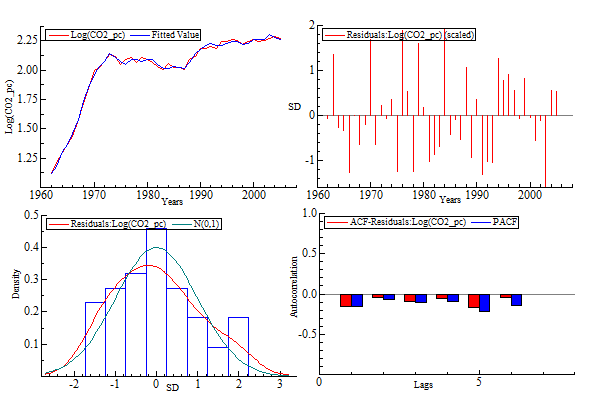
\includegraphics[scale=0.8]{fig2.png}
    \label{fig2} 
  \end{center}
\end{figure}


\begin{table}[h]
  \caption{ADF test with the intercept and trend}
  \label{adf1}
  \centering
  \begin{tabular}{crr}
    \hline
   Variable  & Std. Error & t-value\\
\hline\hline
$\ln{(CO_2)}$ &   0.043587   &   -3.4192 \\
$\ln{(GDP)}$  & 0.028171     & -2.1910 \\
$(\ln{(GDP)})^2$ &  0.027584 &     -1.8220  \\
$\ln{(ENC)}$ &  0.062286   &   -2.0236 \\
$\ln{(URBP)}$ & 0.017534  &    -2.2748 \\
    \hline
    *$5\%=-3.516$, & **$1\%=-4.184$
  \end{tabular}
\end{table}


\begin{table}[h]
  \caption{ADF test with the intercept and trend}
  \label{adf2}
  \centering
  \begin{tabular}{crr}
    \hline
   Variable  & Std. Error & t-value\\
\hline\hline
$\varDelta{\ln{(CO_2)}}$  & 0.14245  &    -5.0386**\\
$\varDelta{\ln{(GDP)}}$ &    0.14432 &     -4.4211**\\
$\varDelta{(\ln{(GDP)})^2}$ &     0.14561 &     -4.4382**\\
$\varDelta{\ln{(ENC)}}$ &  0.15640  &    -5.7661**\\
$\varDelta{\ln{(URBP)}}$ &    0.082385  &    -3.8725*\\
    \hline
*$5\%=-3.514$,& **$1\%=-4.178$
  \end{tabular}
\end{table}

\newpage

\begin{table}[htbp]
\caption{1-step forecasts for $\varDelta{\ln{(CO_2)}}$ (SE based on error variance only)}
\label{table}
\centering
\begin{tabular}{lrrrrrrr}
\hline
Horizon    &  Forecast  &      SE    &    Actual  &     Error &  t-value   &     -2SE &       +2SE\\
\hline\hline      
      2006  &  -0.0194977 &   0.02027  & -0.00543840 &   0.014059   &  0.694  & -0.060030 &   0.021034\\
      2007  &   0.0316407 &  0.02027  &   0.0158650  & -0.015776 &   -0.778  & -0.0088911  &  0.072173\\
      2008  &  0.00464431 &  0.02027&    -0.0354616&   -0.040106 &   -1.979&   -0.035888 &   0.045176\\
      2009 &   -0.0402035&   0.02027 &   -0.0910229&   -0.050819  &  -2.508  & -0.080735&  0.00032838\\
      2010  &   0.0322875 &  0.02027   &  0.0625572&    0.030270  &   1.494 & -0.0082443  &  0.072819\\
      \hline
\end{tabular}
\end{table}
\begin{table}[htbp]
\begin{tabular}{lrlr}
   mean(Error) = & -0.012474 & RMSE\footnotemark = & 0.033328\\
   SD(Error)   = &   0.03090& MAPE\footnotemark =  &  115.05 \\
\end{tabular}   
\end{table}
\footnotetext{$\displaystyle\sqrt{\frac{1}{k}\sum_{i=1}^{k} \varepsilon^2_{T+i}}$ where $\varepsilon_{T+i}=(\hat y_{T+i|T}-y_{T+i})$}
\footnotetext{$\displaystyle\frac{100}{k}\sum_{i=1}^{k}|\varepsilon_{T+i}|$}

\end{document}